\documentclass{article}

\usepackage{graphicx}
\usepackage{tikz}
\usepackage{tikzsymbols}
\usetikzlibrary{calc,patterns,shapes.geometric}
\pagestyle{empty}
\usepackage[margin=0pt]{geometry}
\geometry{papersize={14in,12in}}

\def\centerarc[#1](#2)(#3:#4:#5){\draw[#1] ($(#2)+({#5*cos(#3)},{#5*sin(#3)})$) arc (#3:#4:#5);}

\begin{document}
	\begin{figure}
		\centering
		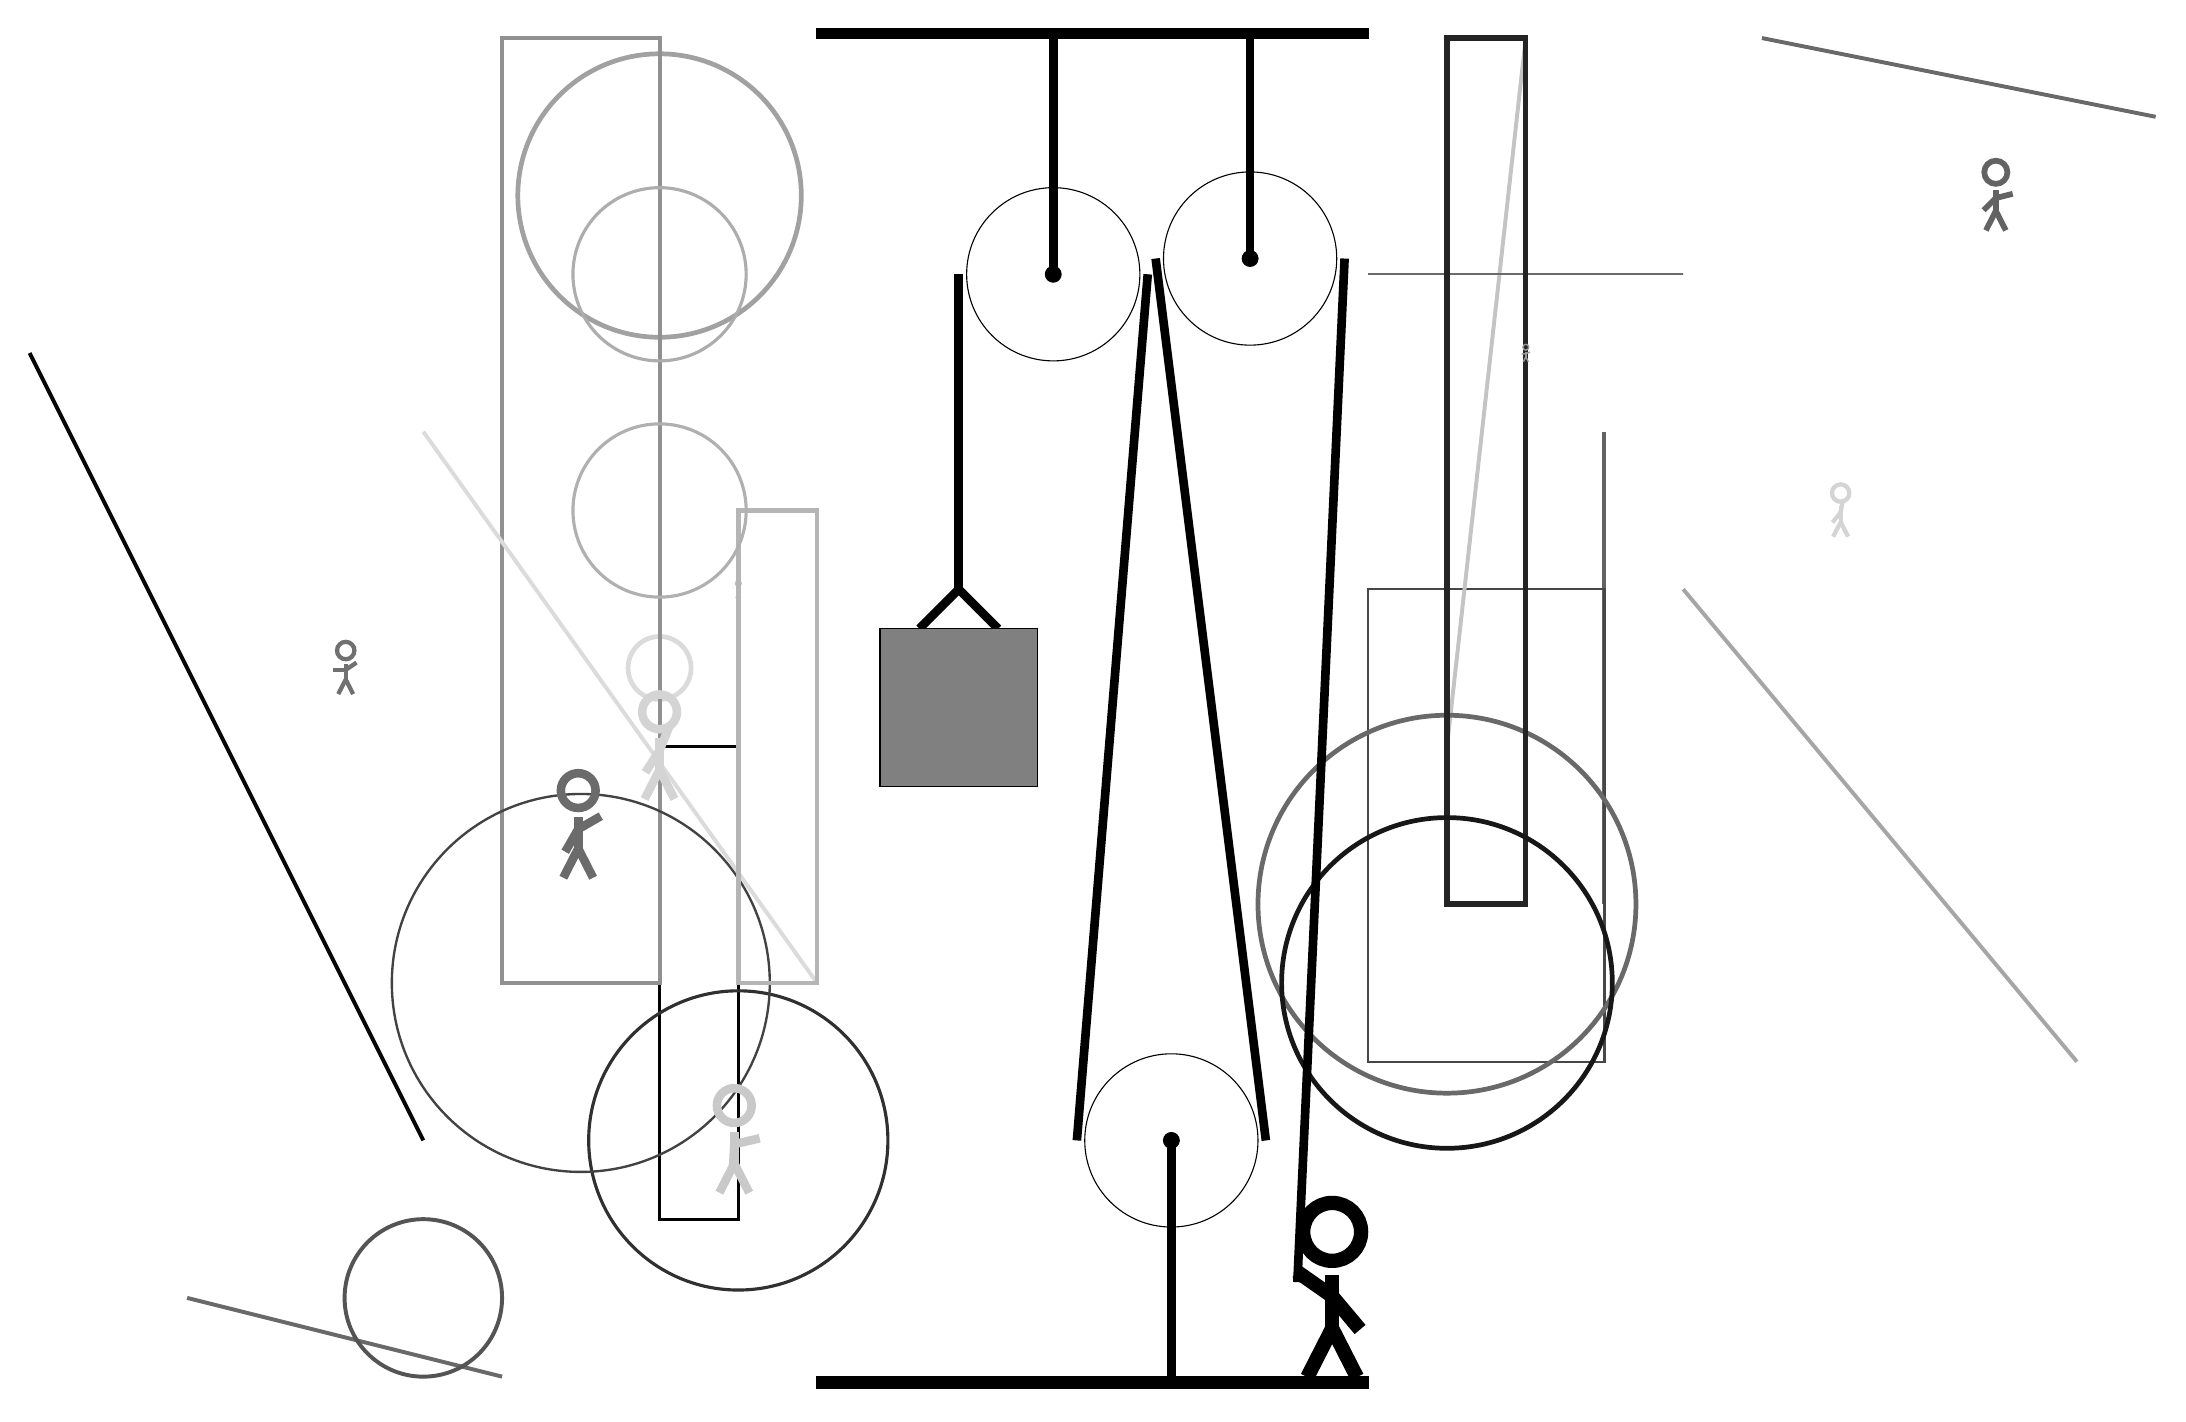
\begin{tikzpicture}
			%%%%% START %%%%%
			
			\draw[fill=black] (-2, 14) rectangle (5, 14.125);
			
			\draw (1, 11) circle (1.1);
			\draw[fill=black] (1, 11) circle (0.1);
			\draw[line width=1.1mm]  (1, 14) -- (1, 11);
			
			\draw[fill=white](2.5, 0) circle (1.1);
			\draw[fill=black] (2.5, 0) circle (0.1);
			\draw[line width=1.1mm]  (2.5, -3) -- (2.5, 0);
			
			\draw[line width=0.5mm, color=black!35](9, 7) -- (14, 1);
			
			\draw [line width=0.6mm, color=black!14](-4, 6) circle (0.4);
			\draw[line width=0.5mm, color=black!59](-6, -3) -- (-10, -2);
			\draw[line width=0.5mm, color=black!92](9, 13) -- (9, 13);
			\draw[line width=0.5mm, color=black!61](8, 9) -- (8, 3);
			\draw[line width=0.5mm, color=black!98](-7, 0) -- (-12, 10);
			\draw[line width=0.4mm, color=black!99] (-3, 5) rectangle (-4, -1);
			\draw[line width=0.3mm, color=black!72] (5, 1) rectangle (8, 7);
			\draw[line width=0.5mm, color=black!23](6, 5) -- (7, 14);
			
			\draw[line width=0.2mm, color=black!58] (5, 11) rectangle (9, 11);
			
			\node[line width=0.5mm, color=black!17] at (11, 8) {\Strichmaxerl[3][51][80]};
			
			\node[line width=0.3mm, color=black!23] at (-3, 7) {\Strichmaxerl[1][70][62]};
			\draw [line width=0.6mm, color=black!37](-4, 12) circle (1.8);
			
			\draw[line width=0.5mm, color=black!43] (-4, 2) rectangle (-6, 14);
			\draw [line width=0.6mm, color=black!59](6, 3) circle (2.4);
			\draw [line width=0.4mm, color=black!81](-3, 0) circle (1.9);
			\node[line width=0.2mm, color=black!61] at (13, 12) {\Strichmaxerl[4][45][14]};
			\draw [line width=0.4mm, color=black!32](-4, 11) circle (1.1);
			\draw [line width=0.3mm, color=black!74](-5, 2) circle (2.4);
			
			\draw[line width=0.5mm, color=black!14](-7, 9) -- (-2, 2);
			\draw [line width=0.5mm, color=black!67](-7, -2) circle (1.0);
			
			\node[line width=0.5mm, color=black!58] at (-5, 4) {\Strichmaxerl[6][60][30]};
			\draw[line width=0.7mm, color=black!86] (7, 14) rectangle (6, 3);
			\node[line width=0.5mm, color=black!17] at (-4, 5) {\Strichmaxerl[6][57][68]};
			\draw[line width=0.5mm, color=black!59](10, 14) -- (15, 13);
			
			\draw[line width=0.6mm, color=black!29] (-3, 8) rectangle (-2, 2);
			
			\draw [line width=0.4mm, color=black!31](-4, 8) circle (1.1);
			\draw [line width=0.6mm, color=black!91](6, 2) circle (2.1);
			\node[line width=0.3mm, color=black!40] at (7, 10) {\Strichmaxerl[1][6][21]};
			\node[line width=0.5mm, color=black!21] at (-3, 0) {\Strichmaxerl[6][87][13]};
			\node[line width=0.5mm, color=black!56] at (-8, 6) {\Strichmaxerl[3][0][34]};
			
			
			\draw[fill=white](3.5, 11.2) circle (1.1);
			\draw[fill=black] (3.5, 11.2) circle (0.1);
			\draw[line width=1.1mm] (3.5, 14) -- (3.5, 11.2);
			
			\draw[line width=1.1mm] (-0.7, 6.5) -- (-0.2, 7.0) -- (0.3, 6.5);
			\draw[fill=black!50] (-1.2, 6.5) rectangle (0.8, 4.5);
			
			\draw[line width=1.1mm] (-0.2, 11) -- (-0.2, 7.0);
			\centerarc[line width=1.1mm](1, 11)(0:180:1.2000000000000002);
			\draw[line width=1.1mm](2.2, 11) -- (1.3, 0);
			\centerarc[line width=1.1mm](2.5, 0)(180:360:1.2000000000000002);
			\draw[line width=1.1mm](3.7, 0) -- (2.3, 11.2);
			\centerarc[line width=1.1mm](3.5, 11.2)(0:180:1.2000000000000002);
			\draw[line width=1.1mm](4.7, 11.2) -- (4.1, -1.8);
			
			\node at (4.5, -1.9) {\Strichmaxerl[10][-35][-50]};
			
			\draw[fill=black] (-2, -3) rectangle (5, -3.15);
			
			%%%%% END %%%%%
		\end{tikzpicture}
	\end{figure}	
\end{document}